\subsubsection{Komponenten}
Komponenten erlauben es in der Benutzeroberfläche wiederverwendbare Teile zu verwenden. Komponenten akzeptieren Eingaben, die „props“ genannt werden, und geben React-Elemente zurück.\cite{komponenten}


In der App werden folgende Komponenten verwendet:

\paragraph{Box}

Hiermit können die aktuell gelagerten Gegenstände oder vergangene Buchungen angezeigt werden. Angezeigt wird der Name des Einlagerungsortes, ein Icon (entweder ein Fahrrad oder Boxen) und das Datum der Einlagerung. Falls die Buchung zu Ende ist, wird außerdem das Enddatum angezeigt.\\

\begin{figure}[H]
    \centering
    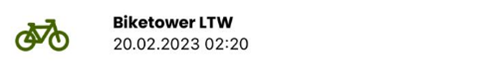
\includegraphics[width=0.4\textwidth]{images/app-screenshots/boxwithbike.png}
    \caption{Komponente Box mit Fahrrad}
    \label{fig:boxwithbike}
\end{figure}
\begin{figure}[H]
    \centering
    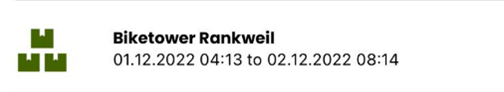
\includegraphics[width=0.4\textwidth]{images/app-screenshots/boxwithitem.png}
    \caption{Komponente Box mit Gegenstand}
    \label{fig:boxwithitem}
\end{figure}

Die Komponente wird auf den Seiten „Aktivität“ und „Fahrradturm“ verwendet. Dafür wird der folgende Code benutzt:\\

\begin{minted}{js}
   <Box navigation={navigation} boxinfo={item} />
\end{minted}

Verwendete Props:
\begin{itemize}
    \item Element für Navigation (navigation)
    \item Array der Box (boxinfo)
\end{itemize}

\paragraph{SettingLink}Mit der Komponente SettingLink erstellt man einen Link, mit dem man zu einer Unterseite mit Einstellungen kommt. Die Komponente wird auf der Seite „Einstellungen“ verwendet.\\

\begin{figure}[H]
    \centering
    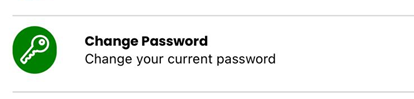
\includegraphics[width=0.4\textwidth]{images/app-screenshots/settinglink.png}
    \caption{Komponente SettingLink}
    \label{fig:settinglink}
\end{figure}

Code zum Erstellen der Komponente SettingLink:\\
\begin{minted}{js}
    <SettingLink
        navigation={navigation}
        navigate={"notdone"}
        picturename="key-outline"
        heading="Change Password"
        info="Change your current password"
      />
 \end{minted}
Verwendete Props:
\begin{itemize}
    \item Element für Navigation (navigation)
    \item Screen auf den navigiert wird (navigate)
    \item Name des Bildes (picturename)
    \item Text der Überschrift (heading)
    \item Text der Info (info)
\end{itemize}


\paragraph{OtherLink}Die Komponente OtherLink funktioniert ähnlich wie die Komponente SettingLink. Sie wird auf dem Screen Services verwendet. Die Komponente dient als Link zu Unterseiten.\\
\begin{figure}[H]
    \centering
    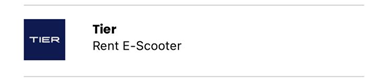
\includegraphics[width=0.4\textwidth]{images/app-screenshots/otherlink.png}
    \caption{Komponente OtherLink}
    \label{fig:otherlink}
\end{figure}
Code zum Erstellen der Komponente OtherLink:\\
\begin{minted}{js}
    <OtherLink
        navigation={navigation}
        navigate={"qr"}
        picturename={require("./../assets/images/tierlogo.jpg")}
        heading="Tier"
        info="Rent E-Scooter"
      />
\end{minted}
Verwendete Props:
\begin{itemize}
    \item Element für Navigation (navigation)
    \item Screen auf den navigiert wird (navigate)
    \item Link zum Bild (picturename)
    \item Text der Überschrift (heading)
    \item Text der Info (info)
\end{itemize}


\paragraph{BoxImage}Die Komponente BoxImage wird auf dem Screen „Assignment“ und „BoxInfo“ verwendet. Die Komponente rendert ein Bild der Box entweder mit einem Fahrrad oder mit Boxen, je nachdem ob die Variable type „bike“ oder „item“ lautet.\\
\begin{figure}[H]
    \centering
    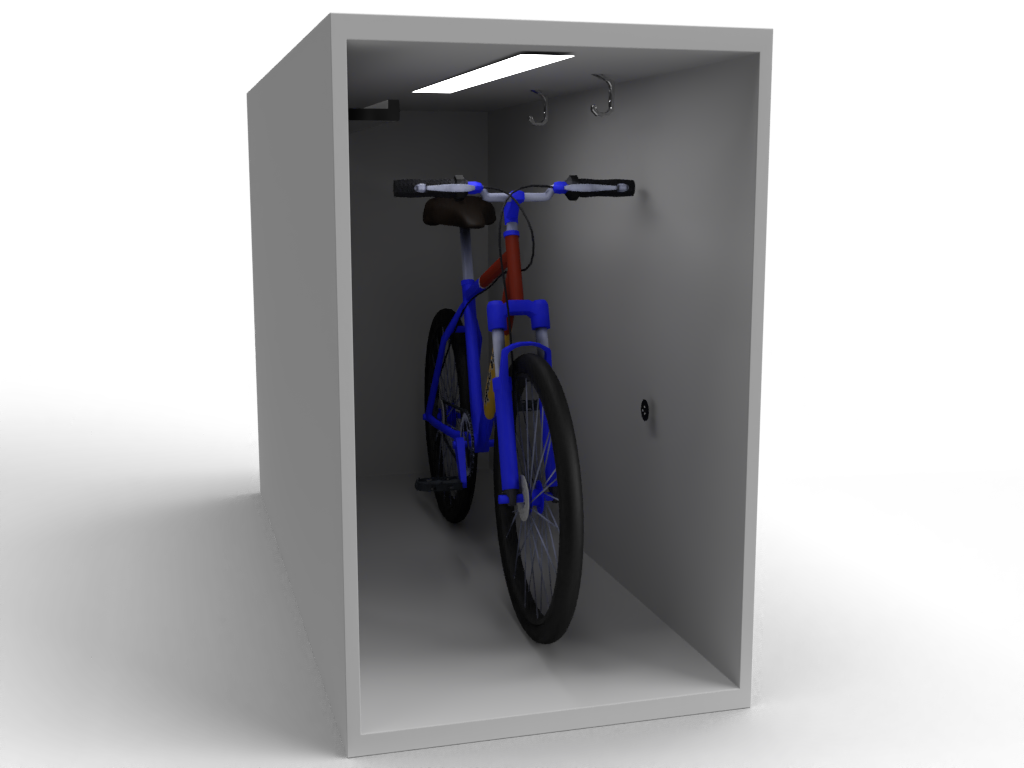
\includegraphics[width=0.4\textwidth]{images/box_bike.png}
    \caption{Komponente BoxImage als Fahrradbox}
    \label{fig:boximagebike}
\end{figure}
\begin{figure}[H]
    \centering
    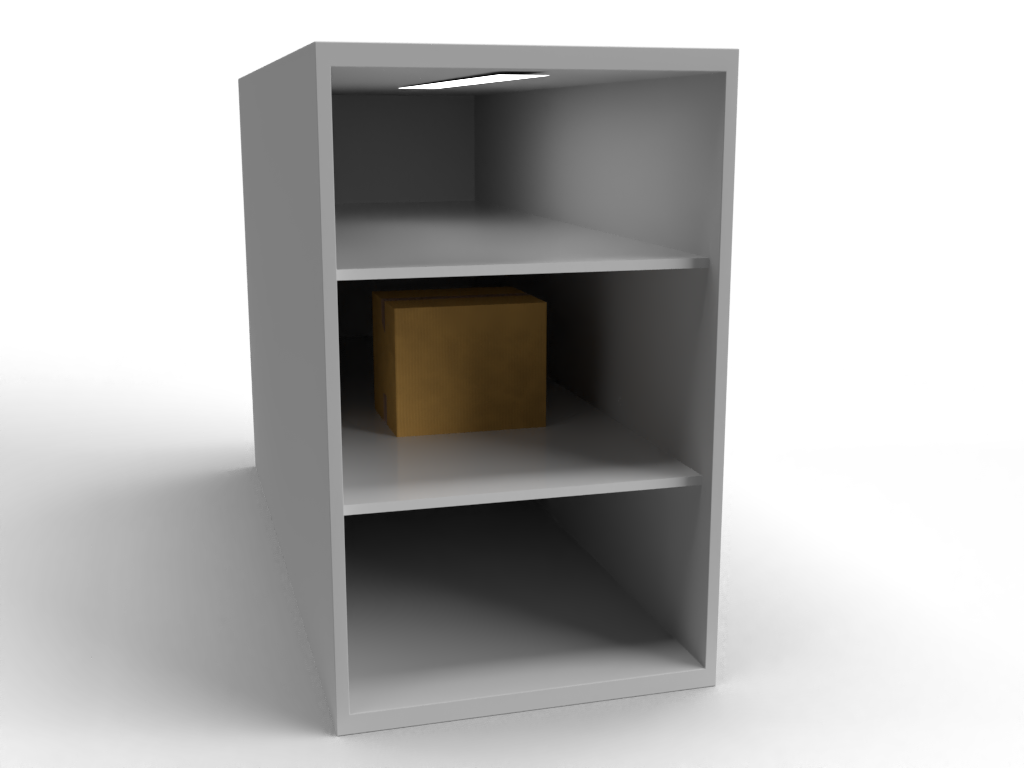
\includegraphics[width=0.4\textwidth]{images/box_item.png}
    \caption{Komponente BoxImage als Box für Gegenstände}
    \label{fig:boximageitem}
\end{figure}
Code zum Erstellen der Komponente BoxImage:\\
\begin{minted}{js}
    <BoxImage type={box.boxref.type}/>
\end{minted}
Verwendete Props:
\begin{itemize}
    \item Art der Box (type)
\end{itemize}
